% !TEX root=/home/tavant/these/manuscript/src/manuscript.tex

\section{Secondary electron emission}

When an incident electron reaches the wall material, several scenarii are possible, as described in \citet{villemant}
\begin{enumerate}
  \item Elastic reflection: the electron encounter only elastic collision with the material, hence its energy is constant. However, its direction is not necessary specular.
  \item Inelastic reflection: the electron loose some of its energy to the material.
  \item Secondary electron emission: the energy of the primary electron is enough to extract one or more electrons from the material.
  \item No emission, the electron is absorbed by the wall.
\end{enumerate}

The probability \proba  that one event appends instead of the other depends predominantly on the particle energy, and weakly on its  impact angle.
Concerning the mean flux of electron incident and emitted, we uses the mean emission rate, or yield, \rate.

\subsection{Models of emission } \label{subsec-seemodels}
Several models can be used to describe the electron emission.

\paragraph{Monte Carlo models} are the more realistic.
 They are based on the computation of the trajectory of the electrons through the material, during which the electron can encounter several interactions with the material.
 Each interactions can modify the electron direction, energy, and generate new electron.
 Several models have been proposed, as \citet{furman2002,pierron2017}.
 These models allow a precise characterization of the processes, but depends of a large number of parameters difficult to obtain due to the lack of experimental data.
 
\paragraph{Analytical models} provides a simplified description of the rate of emission.
Their complexity depends of the precision desired.
The more largely used are the models of \citet{vaughan1989,barral2003a,sydorenko2006b}.

In this work, we only are interested in representing qualitatively the electron emission.
Moreover, \citet{croes2017} showed that changing the model used do not affect significantly the results. 
Hence, we will use the model of \citet{barral2003a} for its simplicity.

\subsection{Electron emission model used}
The emission model used in the works follow a linear-saturated law for the probability of emission with three parameters. 
It describes the total emission corresponding to the sum of the elastic and inelastic backscattering and the secondary electron emission.
\begin{equation} \label{eq-proba_barral}
  \proba(\ek) = 
  \begin{cases}
    \proba_0 + (1 - \proba_0) \frac{\ek}{\ek^*}   &\text{ if } \ek < \frac{\probamax - \proba_0}{1 - \proba_0} \ek^*  \\
    \probamax &\text{ if } \ek \geq \frac{\probamax - \proba_0}{1 - \proba_0} \ek^*
  \end{cases}
\end{equation}
where $\ek$ is the kinetic energy of the incoming electron, $\proba_0$ is the asymptotic probability of emission at energy null, $\ek^*$ is the crossover energy above which the probability of emission is higher that one, and \probamax is the maximum probability.
\Cref{eq-proba_barral} is illustrated on \Cref{fig-modelbarral}.

\begin{figure}[hbtp]
  \centering
  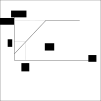
\includegraphics[width=\defaultwidth]{barral}
  \caption{Linear-saturated emission model from \citet{barral2003a}.}
  \label{fig-modelbarral}
\end{figure}

 We suppose that all of the electron emitted are isotropically emitted following a Maxwellian flux distribution function of temperature $\Tsee$.
 The parameters $\proba_0$,  $\probamax$ and $\ek^*$ can be obtained from experiments. 
 \Cref{tab-seeparames} shows the crossover energy and the  probability of emission at energy null for different materials.
 The  asymptotic probability of emission at energy null $\proba_0$ is close to $0.5$, but $\ek^*$ can vary from 18 to 305 V.
 Hence, in the following parametric studies, $\proba_0$ will be kept at 0.5 while we very $\ek^*$ from low values, corresponding to highly emmissive materials, to high values, representing less emmissive materials.
 
 \begin{table}[hbtp]
   \ra{1.3}
   \centering
   \caption{Emission parameters for different material, from \citet{barral2003a}.}
   \label{tab-seeparames}
   \begin{tabular}{@{}lll@{}} \toprule
   Material & $\ek^*$ (V)& $\proba_0$ \\ \midrule
   BN-SiO$_2$ & 53 & 0.45 \\ 
   Al$_2$O$_3$ & 18  & 0.57 \\ 
   SiC     &  43  &0.69  \\
   Graphite & 305  & 0.40 \\ 
   \bottomrule
   \end{tabular}
 \end{table}
 


\section{Conclusion}
  \label{sec-conclusion_ch1}
  
  In order to study the plasma wall interaction in an \ac{HET}, we developed a bi-dimensional simulation code using \ac{PIC}-\ac{MCC} modeling.
  As the electrons drift azimuthally due to the $E \times B$ configuration, the \ac{ECDI} rises, enhancing the cross field transport of the electron toward the anode.
  The walls closing the chamber in the radial direction are also important for the discharge behaviour.
  Hence, in order to compare the interaction between these phenomena, we simulate the radial-azimuthal domain.
  
  A special care have been taken concerning
  \begin{itemize}
    \item the modeling of the axial convection, in order to model the energy losses and so attain a steady state,
    \item the modeling of the radial boundary with the dielectric layer included in the simulation domain.
  \end{itemize}
  
  \inlinenote{Add a {\it typical result} to describe the may behaviour of the simulation ?}
  
  